%\UseRawInputEncoding
\documentclass{article}
\setcounter{secnumdepth}{0}
\usepackage[T1]{fontenc}
\usepackage[utf8]{inputenc}
%\usepackage[latin1]{inputenc}
%\usepackage[english, norsk]{babel}
\usepackage{filecontents}
\usepackage{tcolorbox}
\usepackage{url}
\usepackage{etoolbox}
\usepackage{framed}
\usepackage{framed, color}
\usepackage{xcolor}
\usepackage{mdframed}
\usepackage{float}
\usepackage{gensymb}
\usepackage{amsmath}

\definecolor{Black}{rgb}{0.0, 0.0, 0.0}

%Definer kode
\usepackage{listings}
\usepackage{color}
\definecolor{dkgreen}{rgb}{0,0.6,0}
\definecolor{gray}{rgb}{0.5,0.5,0.5}
\definecolor{mauve}{rgb}{0.58,0,0.82}

\lstset{frame=tb,
extendedchars = true,
texcl=true,
  language=ADA,
  aboveskip=3mm,
  belowskip=3mm,
  showstringspaces=false,
  columns=flexible,
  basicstyle={\small\ttfamily},
  numbers=none,
  numberstyle=\tiny\color{gray},
  keywordstyle=\color{blue},
  commentstyle=\color{dkgreen},
  stringstyle=\color{mauve},
  breaklines=true,
  breakatwhitespace=true,
  tabsize=3
}

\usepackage[colorlinks]{hyperref}
\hypersetup{citecolor=Black}
\hypersetup{linkcolor=Black}
\hypersetup{urlcolor=Black}
\usepackage{cleveref}


\setlength{\parindent}{0em}
\setlength{\parskip}{1em}
%\renewcommand{\baselinestretch}{2.0}

%\renewcommand\thesubsection{\alph{subsection}}

\renewcommand{\figurename}{Figure}
\begin{document}
\author{Kent Odde}
\title{Title}

\maketitle
\thispagestyle{empty}
\begin{center}
\includegraphics[width=\linewidth,height=0.2\textheight,keepaspectratio]{img/USN.png}
\end{center}
\newpage

\tableofcontents

\newpage

\section{Abstract}

This is my submission for the semester project in DDV3101, fall 2020.

%Innholdsfortegnelse
\section{Introduction}
A cache controller is what administrates the cache memory. This assigment consists of implementing the cacache controller design which is specified on page 462, in \textit{Computer organization \& Design: The Hardware/Software Interface}

%Oppgaven
\section{Specifications}

The details of the design will become clear throughout the \textit{Implementation} section, however the key specifications for the cache controller design is as follows:
\begin{itemize}
  \item{Direct mapped}
  \item{Writeback using write allocate}
  \item{Block size: 4 words}
  \item{Cache size 16 Kib}
  \item{32-byte addresses}
\end{itemize}

A direct mapped cache controller means that in order to find the cache address for a memory address, we use this formula:

\begin{equation}
  CacheAddress = (MemoryAddress) \bmod (Number\_of\_blocks\_in\_cache)
\end{equation}

In other words, all the memory addresses which end in the same bits, will be mapped to the same cache address. This reduces overhead and lets us avoid expencive memory translation schemes. In order to know what which actual memory address we have in our cache currently, we check the most significant bits of the address, against the tag in stored in the cache at the index we need.

The fact that our cache is using writeback, means that when the CPU wants to write something to memory, we immediately only write it to the cache. The new values will not be written back to memory, until another memory address needs to take the current occupants place in the cache. This is a more efficient approach than for instance write-through, where we write back to both the memory and the cache every single time. 

The cache is designed as a finite state machine, which can be seen in figure \ref{FSB}


\begin{figure}[H]
 \centering
  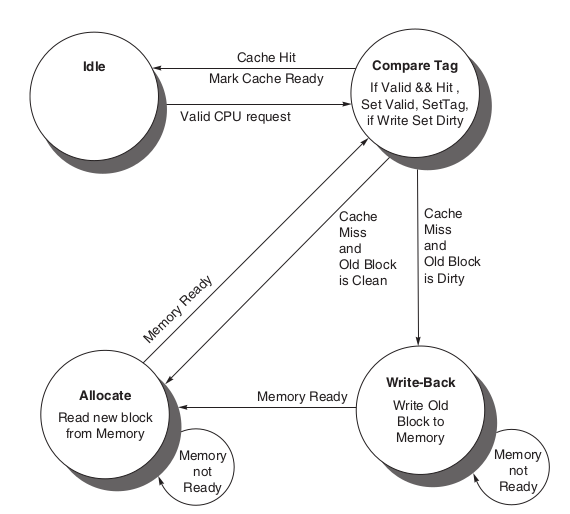
\includegraphics[width=300pt]{img/FSB.png}
  \caption{FSB\cite{BOOK}}
  \label{FSB}
 \end{figure}

An overview of the structure can be seen in figure \ref{OVERVIEW}.

\begin{figure}[H]
 \centering
  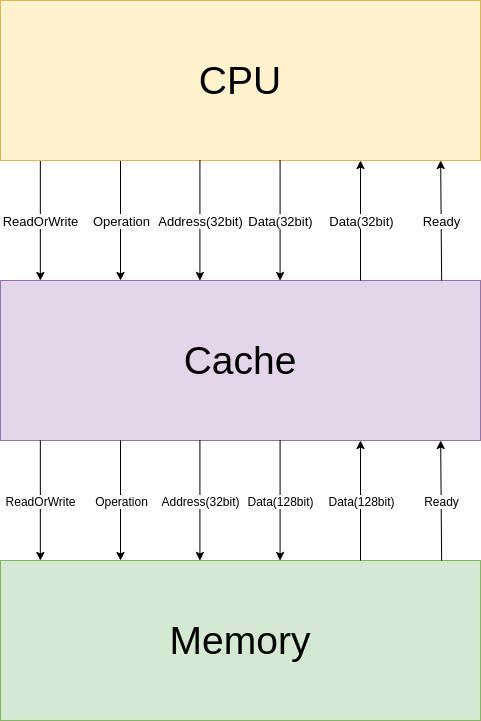
\includegraphics[width=300pt]{img/OverviewBlock.png}
 \caption{Overview}
  \label{OVERVIEW}
 \end{figure}

Lets have a look at how this will work. The CPU will send a 32 bit address to the cache. The cache will go into the state \textit{compare tag}. If we have a cache hit, it will return the correct block over the 32 bit bus to the CPU, and return to its \textit{idle}. However, if we have a miss, it will set the ready bit towards the CPU to 0, and check whether or not the index is valid and dirty. If this is the case, it means that we have to write back data, before we can fetch new the requested memory block into the cache. After the write-back, or if the write-back was not necessary, we move into the \textit{allocate} state, where we request the requested block from memory. The memory will give us 4 blocks on the 128 bit bus between the cache and memory. When this operation is complete, we go back to the \textit{compare tag} state, from where it will naturally return to the \textit{idle} state. 


%Implementation
\section{Implementation}

In order to implement this in VHDL, the cache and the memory will be separate blocks. The ram block will consist of an array to simulate the memory. The cache will consist of one array to store the tags, dirty bits and valid bits, and another array for storing the actual data. 

The CPU in our case will be the testbench, which will request different memory addresses, in order to test all the different outcomes of a memory access. 

The more detailed specifications, can be seen in figure \ref{DETAILED}.

\begin{figure}[H]
 \centering
  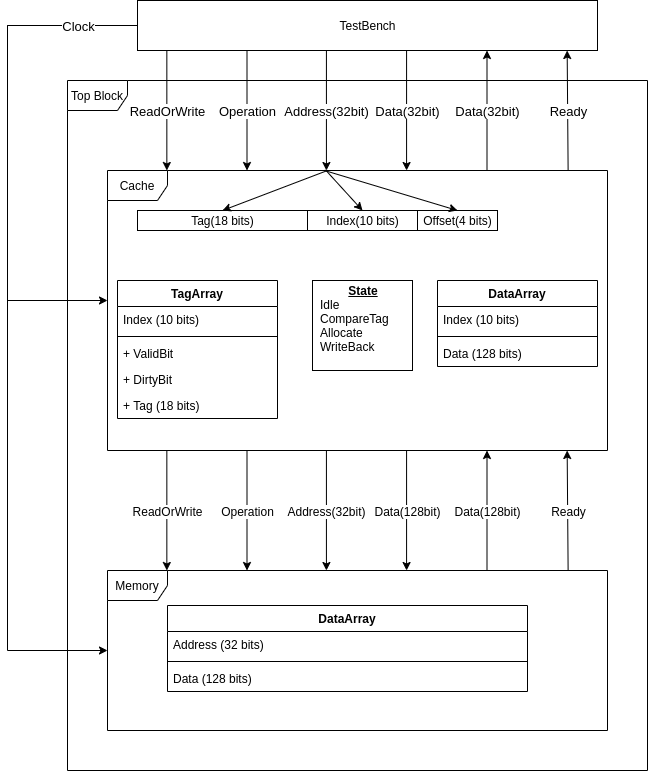
\includegraphics[width=300pt]{img/OverviewDetailed.png}
 \caption{Detailed structure}
  \label{DETAILED}
 \end{figure}




%Konklusjon
\section{Conclusion}




%Vedlegg
\section{Appendices}
\subsection{Testbench}
\begin{lstlisting}
library IEEE;
use IEEE.STD_LOGIC_1164.ALL;

use IEEE.NUMERIC_STD.ALL;

entity TopBlock_tb is
--  Port ( );
end TopBlock_tb;

architecture Behavioral of TopBlock_tb is

    signal clk, ready, operation, readOrWrite : STD_LOGIC;
    signal rData, wData, addr : STD_LOGIC_VECTOR(31 downto 0);

    constant clk_period : time := 10 ns;
    --Define addressess for a more readable testbench
    --First digit refers to the address in decimal, and the second digit means which block we want
    signal address0_0 : std_logic_vector(31 downto 0) := std_logic_vector(to_unsigned(0, 28)) & "0000";
    signal address1_0 : std_logic_vector(31 downto 0) := std_logic_vector(to_unsigned(1, 28)) & "0000";
    signal address1_1 : std_logic_vector(31 downto 0) := std_logic_vector(to_unsigned(1, 28)) & "0100";
    signal address1_2 : std_logic_vector(31 downto 0) := std_logic_vector(to_unsigned(1, 28)) & "1000";
    signal address1_3 : std_logic_vector(31 downto 0) := std_logic_vector(to_unsigned(1, 28)) & "1100";
    signal address2_0 : std_logic_vector(31 downto 0) := std_logic_vector(to_unsigned(2, 28)) & "0000";
    signal address3_0 : std_logic_vector(31 downto 0) := std_logic_vector(to_unsigned(3, 28)) & "0000";
    signal address4_0 : std_logic_vector(31 downto 0) := std_logic_vector(to_unsigned(4, 28)) & "0000";
    signal address5_0 : std_logic_vector(31 downto 0) := std_logic_vector(to_unsigned(5, 28)) & "0000";
    
    signal address1024_0 : std_logic_vector(31 downto 0) := std_logic_vector(to_unsigned(1024, 28)) & "0000";
    signal address1025_0 : std_logic_vector(31 downto 0) := std_logic_vector(to_unsigned(1025, 28)) & "0000";
    signal address1025_1 : std_logic_vector(31 downto 0) := std_logic_vector(to_unsigned(1025, 28)) & "0100";
    signal address1025_2 : std_logic_vector(31 downto 0) := std_logic_vector(to_unsigned(1025, 28)) & "1000";
    signal address1025_3 : std_logic_vector(31 downto 0) := std_logic_vector(to_unsigned(1025, 28)) & "1100";
    signal address1026_0 : std_logic_vector(31 downto 0) := std_logic_vector(to_unsigned(1026, 28)) & "0000";
    signal address1027_0 : std_logic_vector(31 downto 0) := std_logic_vector(to_unsigned(1027, 28)) & "0000";
    signal address1028_0 : std_logic_vector(31 downto 0) := std_logic_vector(to_unsigned(1028, 28)) & "0000";
    signal address1029_0 : std_logic_vector(31 downto 0) := std_logic_vector(to_unsigned(1029, 28)) & "0000";

    constant writeData : std_logic_vector(31 downto 0) := "00001111000011110000111100001111";

    component TopBlock is
    Port (  clk :       in STD_LOGIC := '1';
            ready : out STD_LOGIC := '1';
            operation : in STD_LOGIC := '0';
            rData :     out STD_LOGIC_VECTOR (31 downto 0) := (others => '0');--(Word-1 downto 0);
            addr :      in STD_LOGIC_VECTOR (31 downto 0):= (others => '0');--(AddressBits-1 downto 0);
            wData :     in STD_LOGIC_VECTOR (31 downto 0):= (others => '0');--(Word-1 downto 0);
            readOrWrite :      in STD_LOGIC);
end component TopBlock;



begin
    UUT: TopBlock
    Port Map(    clk => clk, ready => ready, operation => operation, readOrWrite => readOrWrite,
                rData => rData, wData => wData, addr => addr);
                
    
    clk_process : process
    begin
        clk <= '0';
        wait for clk_period/2;
        clk <= '1';
        wait for clk_period/2;
    end process;
    
    
    stim_proc : process
    begin
    --Read from addr0: MISS, 
        wait for clk_period*4;
        readOrWrite <= '0';
        
        wait for clk_period*4;
        addr <= address0_0;
        readOrWrite <= '0';
        operation <= '1';
        wait until ready = '1';
        operation <= '0';
        
        wait for clk_period*4;
        
    --Read from addr0: HIT
        addr <= address0_0;
        readOrWrite <= '0';
        operation <= '1';
        wait until ready = '1';
        operation <= '0';
        
        wait for clk_period*4;
        
    --Write to addr1\_0: MISS, NOT DIRTY
        addr <= address1_0;
        wData <= writeData;
        
        readOrWrite <= '1';
        operation <= '1';
        wait until ready = '1';
        operation <= '0';
        
        wait for clk_period*4;
        
    --Read from addr1\_0: HIT
        addr <= address1_0;
        readOrWrite <= '0';
        operation <= '1';
        wait until ready = '1';
        operation <= '0';
        
        wait for clk_period*4;
        
    --read from addr2\_0: MISS
        addr <= address2_0;
        readOrWrite <= '0';
        operation <= '1';
        wait until ready = '1';
        operation <= '0';
  
        wait for clk_period*4;

    --read from addr1024\_0: CLEAN MISS
        addr <= address1024_0;
        readOrWrite <= '0';
        operation <= '1';
        wait until ready = '1';
        operation <= '0';
        
        wait for clk_period*4;
        
    --read from addr1025\_0: DIRTY MISS
        addr <= address1025_0;
        readOrWrite <= '0';
        operation <= '1';
        wait until ready = '1';
        operation <= '0';
        
        wait for clk_period*4;
        
        
    --Write to addr1\_1: MISS, NOT DIRTY
        addr <= address1_1;
        wData <= writeData;
        readOrWrite <= '1';
        operation <= '1';
        wait until ready = '1';
        operation <= '0';
        
        wait for clk_period*4;
        
        wait;
    end process;

end Behavioral;
\end{lstlisting}
\subsection{Top-Block}
\begin{lstlisting}
library IEEE;
use IEEE.STD_LOGIC_1164.ALL;
use IEEE.Math_real.all;

entity TopBlock is
    Port (  clk :       in STD_LOGIC := '1';
            ready : out STD_LOGIC := '1';
            operation : in STD_LOGIC := '0';
            rData :     out STD_LOGIC_VECTOR (31 downto 0) := (others => '0');
            addr :      in STD_LOGIC_VECTOR (31 downto 0):= (others => '0');
            wData :     in STD_LOGIC_VECTOR (31 downto 0):= (others => '0');
            readOrWrite :      in STD_LOGIC);
end TopBlock;

architecture Behavioral of TopBlock is
    --Constants
    constant Byte : Integer := 8; --(2**3)
    constant Kibi : Integer := 1024; --(2**10)
    constant Word : Integer := 32; --(2**5)
    constant BlockSize : Integer := 4 * Word; --128 (2**7)
    constant CacheSizeBits : Integer := 16 * Kibi * Byte; --16KiB
    constant CacheBlockSize : Integer := CacheSizeBits / BlockSize; --1024 (2**10) 
    constant AddressBits : Integer := 32; --32 Bytes
    constant ValidBitSize : Integer := 1;
    constant DirtyBitSize : Integer := 1;
    constant N : Integer := Integer(log2(Real(CacheBlockSize))); --10
    constant M : Integer := Integer(log2(Real(BlockSize/Word))); -- 2
    
    constant indexSize : Integer := N; -- 10
    constant tagSize : Integer := 18;--32 - (n + m + 2);  --18
    
    constant offsetSize : Integer := 4;
    
    --Output from cacheController
    signal cache2MemReadOrWrite : STD_LOGIC := '0';
    signal cache2MemAddress : STD_LOGIC_VECTOR(addressBits-1 downto 0) := (others => '0');
    signal cache2MemData : STD_LOGIC_VECTOR(BlockSize -1 downto 0) := (others => '0');
    signal cache2MemOperation : STD_LOGIC := '0';
    
    --Output from Memory
    signal mem2CacheReady : STD_LOGIC := '0';
    signal mem2CacheData : STD_LOGIC_VECTOR(BlockSize-1 downto 0) := (others => '0');
    
    --Components
    Component Memory
        Generic(    addressBits : Integer;
                    BlockSize : Integer); 
        Port ( clk :            in STD_LOGIC;
               readOrWrite :    in STD_LOGIC;
               operation :      in STD_LOGIC;
               addr :           in STD_LOGIC_VECTOR (addressBits-1 downto 0);
               --Må være 128 bit:
               dataFromCache :  in STD_LOGIC_VECTOR (BlockSize-1 downto 0);
               dataToCache :    out STD_LOGIC_VECTOR (BlockSize-1 downto 0);
               ready : out STD_LOGIC);
    end Component Memory;
    
    Component Cache
        Generic(    addressBits : Integer;
                    BlockSize : Integer;
                    WordSize : Integer;
                    offsetSize : Integer;
                    indexSize : Integer;
                    tagSize : Integer); 
                  
        Port ( clk :                in STD_LOGIC;
               readOrWriteFromCPU : in STD_LOGIC;
               OperationFromCPU :   in STD_LOGIC;
               addressFromCPU :     in STD_LOGIC_VECTOR(addressBits-1 downto 0);
               dataToCPU :          out STD_LOGIC_VECTOR (Word-1 downto 0);
               dataFromCPU :        in STD_LOGIC_VECTOR (Word-1 downto 0);
               readyToCPU :         out STD_LOGIC;
               
               dataFromMemory :     in STD_LOGIC_VECTOR(BlockSize-1 downto 0);
               dataToMemory :       out STD_LOGIC_VECTOR(BlockSize-1 downto 0);
               addressToMemory :    out STD_LOGIC_VECTOR(addressBits-1 downto 0);
               operationToMemory :  out STD_LOGIC;
               readOrWriteToMemory: out STD_LOGIC := '0';
               readyFromMemory :    in STD_LOGIC);
    end Component Cache; 

begin
    CacheInst : Cache
    Generic Map(addressBits => AddressBits, BlockSize => BlockSize, WordSize => Word, indexSize => indexSize, offsetSize => offsetSize, tagSize => tagSize)
    Port Map(   clk => clk,
                readOrWriteFromCPU => readOrWrite,
                operationFromCPU => operation,
                addressFromCPU => addr, 
                dataToCPU => rData,
                dataFromCPU => wData, 
                readyToCPU => ready,
                dataFromMemory => mem2CacheData,
                dataToMemory => cache2MemData, 
                addressToMemory => cache2MemAddress,
                operationToMemory => cache2MemOperation,
                readOrWriteToMemory => cache2MemReadOrWrite,
                readyFromMemory => mem2CacheReady);
    
    MemoryInst : Memory
    Generic Map(addressBits => AddressBits, BlockSize => BlockSize)
    Port Map(   clk => clk,
                readOrWrite => cache2MemReadOrWrite,
                operation => cache2MemOperation,
                addr => cache2MemAddress,
                dataFromCache => cache2MemData,
                dataToCache => mem2CacheData,
                ready => mem2CacheReady);
                
end Behavioral;
\end{lstlisting}

\subsection{Cache Controller}
\begin{lstlisting}

\end{lstlisting}

\subsection{RAM}
\begin{lstlisting}
library IEEE;
use IEEE.STD_LOGIC_1164.ALL;

use IEEE.NUMERIC_STD.ALL;

entity Memory is
    Generic(    addressBits : Integer;
                BlockSize : Integer); 
    Port ( clk :            in STD_LOGIC;
           readOrWrite :    in STD_LOGIC;
           operation :      in STD_LOGIC;
           addr :           in STD_LOGIC_VECTOR (31 downto 0);
           --Må være 128 bit:
           dataFromCache :  in STD_LOGIC_VECTOR (127 downto 0);
           dataToCache :    out STD_LOGIC_VECTOR (127 downto 0);
           ready : out STD_LOGIC);
end Memory;

architecture Behavioral of Memory is
    --Vivado won't let me have arrays of the intended size (2**32)-1.
    --This smaller array lets me at least use addresses of the first and second "modulodegree", so I have been able to test the cache. 
    type memory_type is array(0 to (2**16)-1) of std_logic_vector(127 downto 0);
    signal RAM : memory_type := (others => (others => '1'));
begin
    process(clk, operation, readOrWrite, addr)
    begin
        if(operation = '1') then
            ready <= '0';
            case readOrWrite is
                when '0' => 
                    dataToCache <= RAM(to_integer(unsigned(addr(31 downto 4))));
                when others =>
                    RAM(to_integer(unsigned(addr(31 downto 4)))) <= dataFromCache;
            end case;
        end if;
        ready <= '1';
    end process; 
end Behavioral;
\end{lstlisting}

\subsection{Mux}
\begin{lstlisting}
library IEEE;
use IEEE.STD_LOGIC_1164.ALL;

entity FourToOneMux is
    Generic (BlockSize : Integer;
                WordSize : Integer);
    Port ( i0 : in STD_LOGIC_VECTOR (BlockSize - 1 downto 0);
           sel : in STD_LOGIC_VECTOR (1 downto 0);
           Y : out STD_LOGIC_VECTOR (WordSize - 1 downto 0));
end FourToOneMux;

architecture Behavioral of FourToOneMux is

begin
    
    Y <=    i0(127 downto 96) when sel = "00" else
            i0(95 downto 64) when sel = "01" else
            i0(63 downto 32) when sel = "10" else
            i0(31 downto 0);
end Behavioral;
\end{lstlisting}
\newpage
%Referanse
%\section{Referanser}

\nocite{*}
\bibliographystyle{plain}
\bibliography{ref}

\addcontentsline{toc}{section}{References}

\end{document}
